\documentclass[tikz]{standalone}
    \usepackage{tikz}
    \usetikzlibrary{positioning, graphs}
    \usetikzlibrary{graphs.standard}
    \begin{document}
    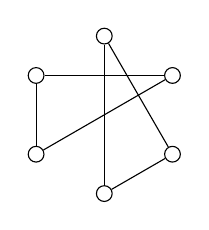
\begin{tikzpicture}
            [every node/.style={draw,circle,inner sep = 0mm, minimum size = 2mm}]
            \graph[clockwise, radius = 1cm, empty nodes]{subgraph I_n[n = 6, name = A]};

            \draw (A 1) -- (A 3);
            \draw (A 1) -- (A 4);
            \draw (A 3) -- (A 4);
            \draw (A 2) -- (A 6);
            \draw (A 2) -- (A 5);
            \draw (A 6) -- (A 5);

            % \foreach \i [evaluate={\j=int(mod(\i+1, 6))+1;}] in {1, 2, 3, 4, 5, 6}{
            %     \draw (A \i) -- (A \j);
            % }
    \end{tikzpicture}
    \end{document}